\documentclass[tikz,border=8pt]{standalone}
\usepackage[T1]{fontenc}
\usepackage{tikz}
\usetikzlibrary{arrows.meta,positioning,calc}

\begin{document}
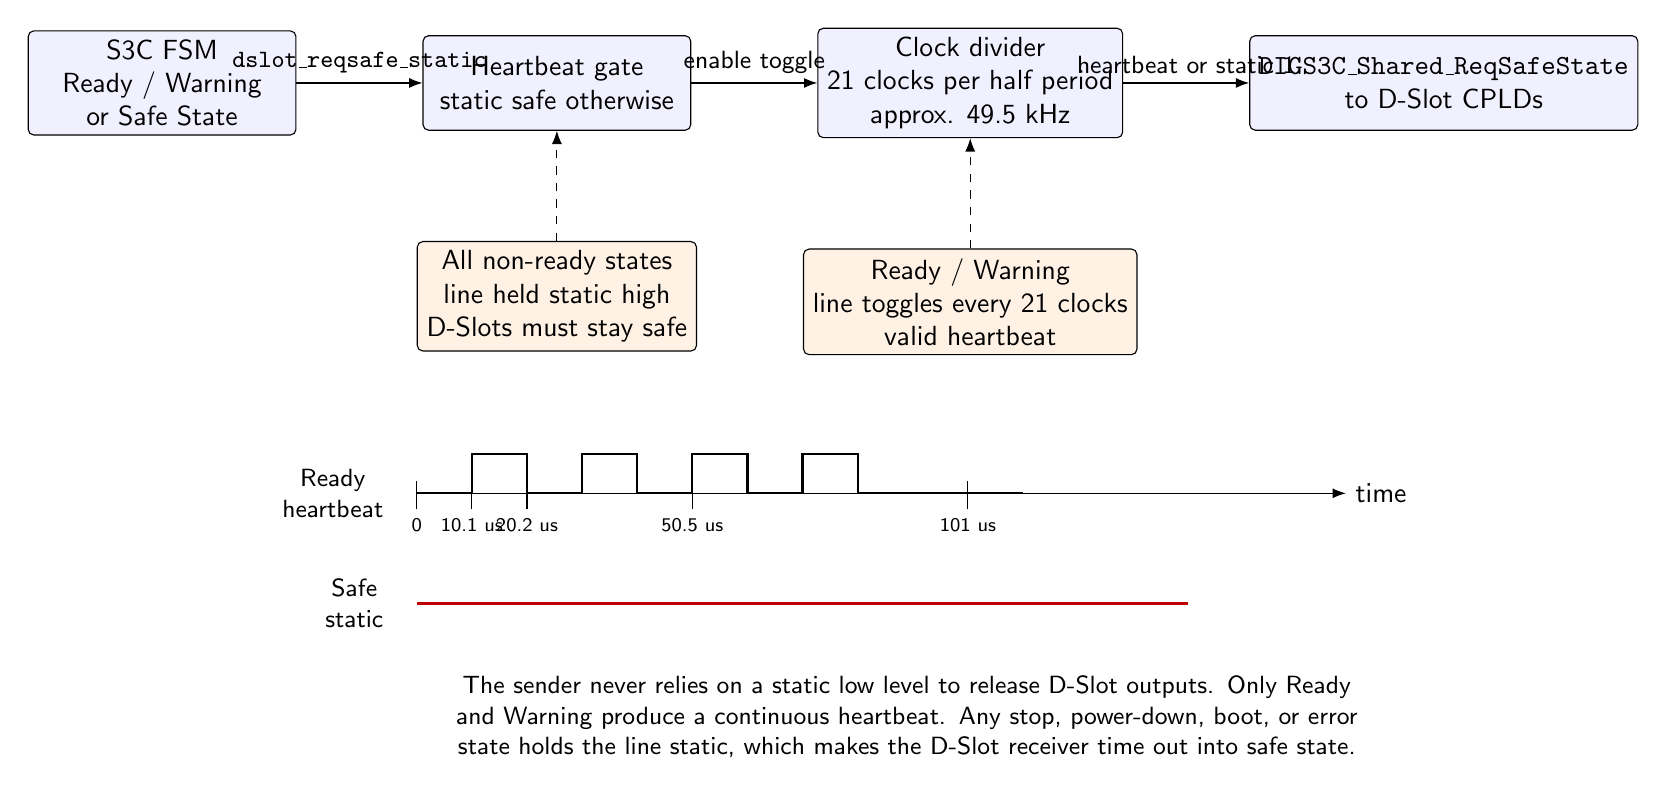
\begin{tikzpicture}[
  font=\sffamily,
  >=Latex,
  block/.style={draw, rounded corners=2pt, align=center, minimum height=12mm, minimum width=34mm, fill=blue!6},
  state/.style={draw, rounded corners=2pt, align=center, minimum height=10mm, minimum width=35mm, fill=orange!10},
  note/.style={align=center, font=\sffamily\small},
  tinytext/.style={align=center, font=\sffamily\scriptsize},
  sig/.style={thick}
]

\node[block] (fsm) {S3C FSM\\Ready / Warning\\or Safe State};
\node[block, right=16mm of fsm] (mux) {Heartbeat gate\\static safe otherwise};
\node[block, right=16mm of mux] (divider) {Clock divider\\21 clocks per half period\\approx. 49.5 kHz};
\node[block, right=16mm of divider] (pin) {\texttt{DIGS3C\_Shared\_ReqSafeState}\\to D-Slot CPLDs};

\draw[->] (fsm) -- node[above,note] {\texttt{dslot\_reqsafe\_static}} (mux);
\draw[->] (mux) -- node[above,note] {enable toggle} (divider);
\draw[->] (divider) -- node[above,note] {heartbeat or static 1} (pin);

\node[state, below=14mm of mux] (safe) {All non-ready states\\line held static high\\D-Slots must stay safe};
\node[state, below=14mm of divider] (ready) {Ready / Warning\\line toggles every 21 clocks\\valid heartbeat};
\draw[->, dashed] (safe) -- (mux);
\draw[->, dashed] (ready) -- (divider);

\coordinate (t0) at ($(safe.south west)+(0,-18mm)$);
\draw[->] (t0) -- ++(118mm,0) node[right] {time};
\node[note, anchor=east] at ($(t0)+(-3mm,0mm)$) {Ready\\heartbeat};
\node[note, anchor=east] at ($(t0)+(-3mm,-14mm)$) {Safe\\static};

\draw[sig] ($(t0)+(0,0)$)
  -- ++(7mm,0) -- ++(0,5mm) -- ++(7mm,0) -- ++(0,-5mm)
  -- ++(7mm,0) -- ++(0,5mm) -- ++(7mm,0) -- ++(0,-5mm)
  -- ++(7mm,0) -- ++(0,5mm) -- ++(7mm,0) -- ++(0,-5mm)
  -- ++(7mm,0) -- ++(0,5mm) -- ++(7mm,0) -- ++(0,-5mm)
  -- ++(21mm,0);
\draw[sig, red!75!black] ($(t0)+(0,-14mm)$) -- ++(98mm,0);

\foreach \x/\lab in {0/0,7/10.1 us,14/20.2 us,35/50.5 us,70/101 us} {
  \draw ($(t0)+(\x mm,1.5mm)$) -- ($(t0)+(\x mm,-2mm)$);
  \node[tinytext, anchor=north] at ($(t0)+(\x mm,-2mm)$) {\lab};
}

\node[note, text width=122mm, below=22mm of t0, anchor=north west] {
The sender never relies on a static low level to release D-Slot outputs. Only Ready and Warning
produce a continuous heartbeat. Any stop, power-down, boot, or error state holds the line static,
which makes the D-Slot receiver time out into safe state.
};

\end{tikzpicture}
\end{document}
